\chapter{Ti-Mo-Nb-Sn-Ta-Zr \\Thermodynamic Database}

\section{Introduction}

The design of Ti-alloys for biomedical applications necessitates a completed thermodynamic database that will facilitate the prediction of phase compositions and fractions as a function of composition and temperature. However, there is no completed thermodynamic database for the Ti-Mo-Nb-Sn-Ta-Zr system and thus the present work aims at building a complete database with special focus on the Ti-rich alloys and bcc phase models. With this in mind the pure elements have been extensively studied and are widely adopted from the SGTE database \cite{Dinsdale1991}. The modeling of the binary systems has been widely documented with the exception of the Ta-Sn and Mo-Sn systems, while experimental phase boundary data is available for the ternary systems but little to no modeling has been completed. The Mo-Sn and Sn-Ta subsystems have high melting temperatures and little to no experimental data. In these cases, first-principles calculations based on DFT can be used to aid in modeling and supplement the lack of experimental data. The complete modeling of the Ta-Sn system is discussed in Chapter 4. In the present chapter, the thermodynamic descriptions of the Ti-Mo-Nb-Sn-Ta-Zr system are described. 

While many of the alloys in this Ti system have been studied experimentally, yielding phase equilibrium data, only limited calorimetry data is available. With the present work focuses on bcc Ti-rich alloys, first-principles calculations based on DFT of the enthalpy of formation of the bcc phase were calculated. The thermodynamic descriptions were built or evaluated using available experimental phase boundary data and present calculated thermochemical data. This works looks at evaluating new and previous models for the binary and Ti-containing ternary systems. 

\section{Computational details}

First-principles results based on Density Functional Theory (DFT) are used to predict the enthalpy of formation of specific phases. In the present work, the enthalpy of formation of the bcc phase was calculated for the Ti-X and Ti-X-Y (X$\neq$Y= Mo, Nb, Sn, Ta, Zr) using the calculated energy of the pure elements in their SER states. For each binary system, 3 special quasirandom structures at different compositions, Ti$_4$X$_{12}$, Ti$_{8}$X$_{8}$, Ti$_{12}$X$_{4}$, were calculated where (X= Mo, Nb, Sn, Ta, Zr). The SQS were each 16-atom supercells that were previously generated and relaxed according to the methodology chapter \cite{Jiang2004}. For each binary system other dilute compositions were calculated, i.e. Ti-Mo 4 dilute structures (Mo$_{53}$Ti 54-atoms, Mo$_{15}$Ti 16-atoms,  Ti$_{7}$Mo 8-atoms, Ti$_{15}$Mo 16-atoms), Ti-Nb 4 dilute structures (Nb$_{53}$Ti 54-atoms, Nb$_{15}$TI 16-atoms, Ti$_{7}$Nb 8-atoms, Ti$_{53}$Nb 54-atoms), Ti-Sn 1 dilute structure (Ti$_{15}$Sn 16-atoms), Ti-Ta 5 dilute structures (Ta$_{53}$Ti 54-atoms, Ta$_{15}$Ti 16-atoms, Ti$_{7}$Ta 8-atoms, Ti$_{15}$Ta 16-atoms, Ti$_{53}$Ta 54-atoms), and Ti-Zr 2 dilute structures (Zr$_{15}$Ti 16-atoms, Ti$_{53}$Zr 54-atoms). For the Ti-X-Y (X $\neq$ Y= Mo, Nb, Sn, Ta, Zr) ternary systems, three SQS calculations were competed at the compositions Ti$_{12}$X$_{12}$Y$_{12}$ (36-atom), Ti$_{16}$X$_{8}$Y$_{8}$ (32-atom), Ti$_{48}$X$_{8}$Y$_{8}$ (64-atom). The ternary SQS were previously generated and also relaxed according to the details outlined in the methodology chapter \cite{Jiang2009}. The DFT calculations are completed using VASP (Vienna ab-initio Simulation Package) \cite{Kresse1996}. The ion-electron interactions were described using the projector augmented wave (PAW) \cite{Kresse1999,Blochl1994} method. Based on the work of comparing X-C functionals (Figure \ref{Ch5-figure:PBEvsPW91}) the exchange-correlation functional of the generalized gradient approach depicted by Perdew, Burke, and Ernzerhof (PBE) was employed \cite{Perdew1996a}. For consistency, a 310 eV energy cutoff was adopted for all calculations, which is roughly 1.3 times higher than the default values suggested by VASP for the elements Ti, Mo, Nb, Sn, Ta, and Zr. The energy convergence criterion was 10$^{-6}$ eV/atom, and the Monkhorst-Pack scheme is used for Brillouin zone sampling \cite{Kresse1996,Monkhorst1976a}. The k-points grid for each calculation are listed in appendix c.

\subsection{Sn binaries and ternaries}

The thermodynamic description of the Mo-Sn system has never been modeled and there is little to no experimental data avaliable. With this fact, first-principles calculations can be used to fill in the missing data points. However, this is not a hugely important sub-system and the modeling will be part of the futrue work. The Ta-Sn system is modeled in chapter 4. For the Sn-Zr system, the thermodynamic description was previously modeled. However, these models do not use compatible sublattice modeling with the current database, for the hcp phase. While the, Sn-Nb and Ti-Sn binary systems have been previously modeled, Sn will only be included in small percentages to the overall Ti-based alloy so until the rest of Sn binaries are modeled Sn will not be included in the database.

\section{Pure element calculation results}

In order to build the Ti-Mo-Nb-Ta-Zr thermodynamic database, thermodynamic descriptions for the all the binary systems are evaluated first for accuracy and model compatibility and incorporated into the database (see Chapter 2). In the present work, only thermodynamic descriptions for the Ti-containing ternary systems are generated, Ti-X-Y (X $\neq$ Y = Mo, Nb, Ta, Zr). When applicable the previous thermodynamic descriptions of the non Ti-containing ternary systems are incorporated into the database. The only case of a thermodynamic description of a non Ti-containing ternary, from this system, available in literature is the Mo-Nb-Ta system \cite{Xiong2004}, and it is incorporated here.

Table \ref{Ch3-table:pspureele} shows the equilibrium properties, volume $V_{0}$, energy $E_{0}$, bulk modulus $B$, and the derivative of bulk modulus $B'$ obtained from Eq. \ref{eq: zeroenergy} at 0 $^{\circ}$K. The energy $E_{0}$ and bulk modulus $B$ are compared with previous first-principles calculations at 0 $^{\circ}$K. The energy values between the present calculations and previous calculations vary by 0 to 0.1 eV/atom. The $B$ results from the present calculations and previous calculations vary by at most 3 GPa. The variances between the $E_{0}$ and $B$ are small and due to the fact that the previous calculations used slightly different input parameters such as a different exchange correlation functional (PBE vs PW91) and higher energy cutoff values. Overall, the results are comparable. The $B$ results from the present calculations at 0 $^{\circ}$K are then compared with experimental values from literature. The variance between the $B$ from the calculations and the $B$ from experiments is also 3 GPa or less. This variance is attributed to the difference in temperature between the calculations and experiments. Based on the small variances shown in Table \ref{Ch3-table:pspureele}, the present calculations are deemed accurate. 


\section{Enthalpy of formation of bcc phase from first-principles}

The enthalpies of formation of the bcc phase (bcc-$H_{Form}$) for the binary and ternary systems are presented in Table \ref{Ch3-table:binaryhform} and Table \ref{Ch3-table:ternhform}, respectively. As discussed in the methodlogy chapter, the bcc-$H_{Form}$ is calculated by Eq. \ref{eq: hform}. It is seen that Table \ref{Ch3-table:binaryhform} shows the first-principles results for bcc-$H_{Form}$ for the Ti-Mo system go from positive to negative to positive indicating the formation of a bcc miscibility gap. The first-principles results of the bcc-$H_{Form}$, for the Ti-Nb, Ti-Ta, and Ti-Zr systems, are positive across the entire composition range. Table \ref{Ch3-table:ternhform} shows the values of the first-principles calculated bcc-$H_{Form}$.  It is seen that the bcc-$H_{Form}$ values, for the Ti-Mo-Nb, Ti-Mo-Ta and Ti-Nb-Ta systems, go from positive at 100 at. \% Ti to negative at 0 at. \% Ti at the X$_{50}$Y$_{50}$ composition. The bcc-$H_{Form}$ values remain positive from 100 at. \% Ti to 0 at. \% Ti at the X$_{50}$Y$_{50}$ composition for the Ti-Mo-Zr, Ti-Nb-Zr, and Ti-Ta-Zr systems. For each system that the bcc-$H_{Form}$ is calculated, the values are compared with the CALPHAD modeling predictions and in some cases, are compared with experimentally obtained results. For some of the systems, when comparing the first-principles results of the bcc-$H_{Form}$ and the CALPAHD modeling prediction of the bcc-$H_{Form}$, no large discrepancies are seen and thus no new modeling is completed. In other cases, comparing the first-principles results of the bcc-$H_{Form}$ and the CALPAHD modeling prediction of the bcc-$H_{Form}$ showed larger discrepancies and then the first-principles bcc-$H_{Form}$ values are used to introduce new bcc interaction parameters. Each binary and Ti-containing ternary system is discussed in detail in the next sub sections below.

\section{Thermodynamic modeling of the ten binary systems}

\subsection{Mo-Nb, Mo-Ta, Nb-Ta}

Figure \ref{Ch3-figure:binary1} shows the calculated phase diagrams for the Mo-Nb, Mo-Ta, and Nb-Ta systems from thermodynamic descriptions in the literature in comparison with experiments. The Mo-Nb, Mo-Ta and Nb-Ta descriptions are adopted from the modeling completed by Xiong et al. \cite{Xiong2004}. Xiong et al. \cite{Xiong2004} modeled these three binary systems and the ternary system, Mo-Nb-Ta. Binary interaction parameters were introduced for the liquid and bcc solution phases. The thermodynamic description, for the Mo-Nb system, was completed using differential thermal analysis experiments that measured both the liquidus and solidus temperatures \cite{Xiong2004}. Xiong et al. \cite{Xiong2004} decided to only use the experiments (shown in Figure \ref{Ch3-figure:binary1} as X and +) that estimated the pure elements melting temperatures reasonably well when evaluating the binary interaction parameters. Xiong et al. \cite{Xiong2004} discussed, that after evaluating the binary interaction parameters for the Mo-Nb system, the experiments, shown by $\circ$, $\bigtriangleup$, $\square$, agreed well with the predicted phase diagram. Even though, the remaining experimental data points ($\diamond$, *) were quite low as compared to the predicted phase diagram, they were also quite low compared to all the other experiments \cite{Xiong2004} and were considered inaccurate. Thus Xiong et al. \cite{Xiong2004} concluded that the thermodynamic description generated is adequate at predicting the experimental data. 

The thermodynamic description, for the Mo-Ta system, was completed using two sets of experimental data ($\bigtriangleup$, *, $\diamond$, $\square$) \cite{Xiong2004}. These particular experimental data points were chosen because they accurately measured the melting temperatures of Mo and Ta. The predicted phase diagram accurately reproduced the experimental data, with the exception of the experimental data \cite{Xiong2004} shown as "$\circ$". This set of experimental data was 70 $^{\circ}$K higher than all other experimental data. So as discussed by Xiong et. al. \cite{Xiong2004} the data were not thought to be accurate and were ignored. 

For the Nb-Ta system, the thermodynamic description was completed using the experimental liquidus data \cite{Xiong2004} depicted in the figure by $\circ$, $\bigtriangleup$, and $\square$, because it predicts the melting temperatures of Nb and Ta accurately. The experimental work which measured the solidus temperature (*) was not used because the melting temperatures of Nb and Ta showed discrepancy. The predicted phase diagram reproduces the experimental data well with the exception of the experimental work depicted by $\diamond$. This data was ignored because the values were 343 $^{\circ}$K higher than the experimental values and thus it was determined by Xiong et al. \cite{Xiong2004} to be inaccurate. The present work agrees with the conclusion reached by Xiong et al. \cite{Xiong2004} and agrees that the phase diagrams reproduce the experimental data accurately. The sublattice models used by Xiong et al. \cite{Xiong2004} are compatible with the working database and the binary descriptions are incorporated without any changes. The interaction parameters for the binary systems incorporated into the database are listed in Table \ref{Ch3-table:ip}. 

\subsection{Mo-Zr, Nb-Zr and Ta-Zr}

Figure \ref{Ch3-figure:binary2} shows the predicted phase diagrams for the Mo-Zr, Nb-Zr, and Ta-Zr systems. For the Mo-Zr system, there are multiple previous thermodynamic descriptions and experimental results available. In the present work, the evaluation by Perez et al. \cite{Perez2003} is chosen to be incorporated due to the fact that their model was also incorporated into the Ti-Mo-Zr ternary modeling found in the literature. The experimental data that is plotted determined the single-phase region, two-phase region, phase boundaries, and peritectic and eutectiod reactions. Perez et al. \cite{Perez2003} went into more details on the available experimental data and discussing what was included in their evaluation. Perez et al. \cite{Perez2003} introduced interaction parameters for the liquid, bcc, hcp, and Laves\_C15 phases. The thermodynamic description generally reproduces all experimental data accurately. 

The thermodynamic description, for the Nb-Zr system, was previously evaluated by Guillermet \cite{Guillermet1991} in the literature. Figure \ref{Ch3-figure:binary2} plots the predicted phase diagram with the solidus experimental data ($\diamond$, *) as well as the hcp solvus (Y, $\circ$) and bcc miscibility gap ($\bigtriangleup$, $\square$, +) data \cite{Guillermet1991,Kumar1994a,Abriata1982}. The description includes interaction parameters for the liquid, bcc, and hcp solution phases and accurately reproduces the experimental data. 

For the Ta-Zr system, the thermodynamic description was also evaluated by Guillermet \cite{Guillermet1995}. As discussed by Guillermet \cite{Guillermet1995}, there is quite a lot of experimental data, phase boundary results from at least five different papers and thermodynamic results from three different papers \cite{Guillermet1995}. Figure \ref{Ch3-figure:binary2} plots the single-phase, two-phase, phase boundary, and solidus experimental data. Interaction parameters were introduced for the bcc, hcp, and liquid phases. The predicted phase diagram reproduces the data fairly well. 

The thermodynamic descriptions of the three binary systems Mo-Zr, Nb-Zr, and Ta-Zr are determined to be accurate and the sublattice modeling used is compatible with the working database. Thus, the thermodynamic descriptions are incorporated into the database. The interaction parameters for the binary systems incorporated into the database are listed in Table \ref{Ch3-table:ip}. 

\subsection{Ti-Mo}

The thermodynamic description in the COST 507 database, modeled by Saunders, \cite{Ansara1998} is looked at for the Ti-Mo system. This model is chosen because it is the model incorporated into the Ti-Mo-Zr thermodynamic modeling \cite{Kar2008}. Interaction parameters were evaluated for the liquid, fcc, hcp, bcc (ordered bcc\#1 and disordered bcc\#2), AlM\_D019, AlM-D022, and the AlTi-L10 phases. Figure \ref{Ch3-figure:TiMo}a plots the predicted phase diagram \cite{Ansara1998} with the available experimental phase boundary data \cite{Murray1981}. The phase boundary data is reproduced accurately. Figure \ref{Ch3-figure:TiMo}b plots the predicted enthalpy of formation of the bcc phase (solid line) versus the results from the present first-principles calculations (circles) and are compared to the enthalpies of formation of the bcc phase obtained experimentally (red squares) \cite{Uesugi2013}. The experimental bcc-$H_{Form}$ values and the prediction from the model are at 300 $^{\circ}$K while the first-principles results are at 0 $^{\circ}$K. The experimental values of bcc-$H_{Form}$ compare well with the calculations but get more negative closer to the Mo-rich side which can be attributed to the temperature difference. The enthalpy of formation of the bcc phase predicted varies from the first-principles calculations drastically between 20 and 80 at.\% Mo. This discrepancy is due to the disagreement on the existence of a bcc miscibility gap. Previous experimental research, including the values plotted here, have shown an equilibrium bcc miscibility gap which would fit what is seen in the first-principles calculations \cite{Uesugi2013,Predel1997,Hoffman1967}. While there is an interaction parameter for the bcc order and disorder, Saunders \cite{Ansara1998} did not model the bcc miscibility gap as being an equilibrium phase. While there are previous thermodynamic descriptions that model the bcc miscibility gap, Kar et al. \cite{Kar2008} showed that the experimental data from higher-component systems fit better with the description containing no miscibility gap. Based on this and the fact that the sublattice modeling is compatible with the working database, the thermodynamic description by Saunders \cite{Ansara1998} is adopted with no changes. The interaction parameters for the binary system incorporated into the database are listed in Table \ref{Ch3-table:ip}.


\subsection{Ti-Nb}

For the Ti-Nb system, its thermodynamic description is taken from Zhang et al. \cite{Zhang2001}. Originally the thermodynamic description by Kumar et al. \cite{Kumar1994,Kumar1994a} was evaluated because it was used in the modeling of the Ti-Nb-Zr system. However, new experimental phase boundary data on the Nb rich side ($\bigtriangleup$) showed the need to switch to the Zhang et al. \cite{Zhang2001} thermodynamic description. Zhang et al. \cite{Zhang2001} introduced interaction parameters for the Liquid, bcc, hcp and omega phases. Figure \ref{Ch3-figure:TiNb}a plots the predicted phase diagram from Zhang et al. \cite{Zhang2001} versus solidus data ($\square$), hcp and bcc solvus data ($\circ$) \cite{Kumar1994,Kumar1994a} and the new Nb-rich bcc solvus data ($\bigtriangleup$) \cite{Zhang2001}. Figure \ref{Ch3-figure:TiNb}b plots the predicted enthalpy of formation (solid line) versus the present first-principles calculations (circles) and are compared to the enthalpies of formation of the bcc phase obtained experimentally (red squares) \cite{Uesugi2013}. The experimental bcc-$H_{Form}$ values and the prediction from the model are at 300 $^{\circ}$K while the first-principles results are at 0 $^{\circ}$K. The experimental bcc-$H_{Form}$ values compare well with the calculations and any variance can be attributed to the temperature difference. There is an average variance of 0.17 kJ/mol-atom between the DFT and CALPHAD predictions of th bcc-$H_{Form}$ which is also attributed to the temperature difference. However, even with the variance, the CALPHAD prediction compares well with the DFT results and the phase diagram reproduces the experimental data accurately. The sublattice models are compatible and the thermodynamic description from Zhang et al. \cite{Zhang2001} is incorporated into the present database with no alterations. The interaction parameters for the binary system incorporated into the database are listed in Table \ref{Ch3-table:ip}.

\subsection{Ti-Ta}

The thermodynamic description, for the Ti-Ta system, is taken from the COST 507 database \cite{Ansara1998}. The predicted phase diagram is plotted in Figure \ref{Ch3-figure:TiTa}a, with the experimental liquidus and solidus data ($\diamond$ and Y) as well as bcc and hcp solvus data ($\bigtriangleup$, $\square$, and $\circ$) for comparison. The evaluation includes interaction parameters for the fcc, hcp, liquid, AlM-D019, AlM-D022, AlTi-L10, and the bcc (ordered bcc\#1, disordered bcc\#2) phases \cite{Murray1987}. The thermodynamic description reproduces the experimental data accurately. The enthalpy of formation of the bcc phase predicted by the CALPHAD modeling (solid line) is plotted with the first-principles results (circles) in Figure \ref{Ch3-figure:TiTa}b. The CALPHAD prediction of the bcc-$H_{Form}$ reproduces the results from first-principles reasonably well on the Ti-rich and Ta-rich sides. The first-principles results vary on an average by 0.17 kJ/mol-atom. However, the CALPHAD prediction is at 300 $^{\circ}$K and the first-principles are at 0 $^{\circ}$K which explains the variance. Based on these conclusions the thermodynamic description is deemed accurate and since the sublattice modeling is compatible, the thermodynamic description is incorporated into the database and not altered. The interaction parameters for the binary system incorporated into the database are listed in Table \ref{Ch3-table:ip}.

\subsection{Ti-Zr}

The thermodynamic description, of the Ti-Zr system, evaluated by Kumar et al. \cite{Kumar1994a} is used in the present work. The model by Kumar et al. is chosen because it was used in the ternary modeling of the Ti-Mo-Zr and Ti-Nb-Zr systems. The evaluation introduces interaction parameters for the liquid, bcc, and hcp solution phases. Figure \ref{Ch3-figure:TiZr}a plots the predicted phase diagram compared with phase boundary data for the bcc to hcp ($\circ$) phase transformation and solidus ($\bigtriangleup$). The thermodynamic description accurately reproduces the phase boundary data. When doing the evaluation, heat of transformation data was also used and was discussed by Kumar et al. \cite{Kumar1994a}. Figure \ref{Ch3-figure:TiZr}b plots the present first-principles results (circles) versus the CALPHAD prediction (solid line) for the bcc-$H_{Form}$. The first-principles results and CALPHAD modeling vary on average by 1.2 kJ/mol-atom. The variance is larger than the other binary alloys due to the instability of the bcc phase at both 0 $^{\circ}$K and 300 $^{\circ}$K for the Ti-Zr alloy but the calculations and CALPHAD prediction follow the same trend. Based on the agreement between the experimental data, no alterations were made to the thermodynamic description and with the sublattice modeling compatibility, it was incorporated into the database. The interaction parameters for the binary system incorporated into the database are listed in Table \ref{Ch3-table:ip}. 

\section{Thermodynamic modeling of six Ti-containing ternary systems}

\subsection{Ti-Mo-Nb}

A thermodynamic description, for the Ti-Mo-Nb system, has never been evaluated in the literature. Two experimental investigations were done on the Ti-Mo-Nb system at 873 $^{\circ}$K and 1373 $^{\circ}$K \cite{English1961,Prokoshkin1967}. While both investigations agree that the isothermal section at 1373 $^{\circ}$K is solely the bcc phase, the investigations differed on the phase boundary at 873 $^{\circ}$K. It is suspected that at such a low temperature the samples did not reach equilibrium which accounts for the discrepancy. Based on this, the binary interpolation of the isothermal sections at 1373 $^{\circ}$K and 873 $^{\circ}$K are plotted. The predicted phase diagram at 1373 $^{\circ}$K agreed with the experimentally determined phase diagram to be solely the bcc phase. The phase diagram at 873 $^{\circ}$K is plotted in Figure \ref{Ch3-figure:TiMoNb}a. The discrepancy, at 873 $^{\circ}$K, is the existence of the bcc miscibility gaps as well as what compositions the phase boundary lines lie at. The enthalpy of formation of the bcc phase is predicted using an interpolation of the binary interaction parameters (solid line) and plotted with the first-principles results, in Figure \ref{Ch3-figure:TiMoNb}b, starting from a 50-50 mixture of the alloying elements (Mo$_{50}$Nb$_{50}$) to 100 at.\% Ti. While the first-principles calculations are at 0 $^{\circ}$K and the binary interpolation is at 300 $^{\circ}$K, the calculation results are reproduced with the CALPHAD prediction. The prediction varies by less than 1.5 kJ/mol-atom for all the calculations except at Mo$_{50}$Nb$_{50}$. While the calculation varies substantially from the prediction at Mo$_{50}$Nb$_{50}$, in order to improve this, the Mo-Nb binary system would have to be adjusted. In the present work, no thermochemical data was used to ensure the accuracy of the non Ti-containing binary systems but the previous binary models were able to reproduce the phase boundary data as discussed above. Based on the discrepancy between the experimental data and the fact that the first-principles thermochemical calculations are reproduced well by the binary interpolation, no ternary interaction parameters are evaluated. 


\subsection{Ti-Mo-Ta}

The thermodynamic description, of the Ti-Mo-Ta system, has not been previously modeled. The binary interpolation of the Ti-Mo-Ta alloy is plotted in Figure \ref{Ch3-figure:TiMoTa1}a at 873 $^{\circ}$K. At 873 $^{\circ}$K, the Ti-Mo-Ta alloy has the bcc and hcp solution phases with at tie triangle showing a three-phase region of bcc\#1, bcc\#2, and hcp. The experimental data agreed with the two-phase bcc-hcp region in the Ti-rich corner, but did not see a bcc miscibility gap or tie triangle \cite{Nikitin1971}. Figure \ref{Ch3-figure:TiMoTa1}b shows the present first-principles calculations (circles) of the bcc-$H_{Form}$ compared with the binary interpolation from the CALPHAD prediction (solid black line). The first-principles calculations line up fairly well with the CALPHAD prediction. However, due to the discrepancy of the experimental data ternary interaction parameters are investigated for the hcp and bcc phases using the first-principles results and experimental phase boundary data. The evaluated interaction parameters are listed in Table \ref{Ch3-table:ip}. After assessing the ternary interaction parameters, the isothermal section at 873 $^{\circ}$K is again plotted and compared with experimental data in Figure \ref{Ch3-figure:TiMoTa2}a and zoomed in for Figure \ref{Ch3-figure:TiMoTa2}b. The enthalpy of formation of the newly assessed bcc phase is plotted as a red dashed line in Figure \ref{Ch3-figure:TiMoTa1}b. The assessment reproduces the first-principles results accurately. With the introduction of the interaction parameters the isothermal section fits with the experimental data \cite{Nikitin1971}. The work by Nikitin \cite{Nikitin1971} determined hcp phase boundary data plotted as $\circ$ and two phase experimental data as $\LEFTcircle$. The two phase experimental data is reproduced by the present model. The hcp phase boundary data are not reproduced. However, reliable solid phase boundary data are difficult to obtain at such a low temperature and if the evaluation is altered to fit the data; it then over fits and stabilizes non-equilibrium phases. 

\subsection{Ti-Mo-Zr}

The thermodynamic description of the Ti-Mo-Zr system was previously modeled by Kar et al. \cite{Kar2008}. The same binary phases used in the modeling by Kar et al. are included in the present database. The phases in this ternary system are liquid, bcc, hcp, and Laves\_C15. After interpolating the ternary system from the binary models and comparing to two sets of available experimental data, Kar et al. \cite{Kar2008} introduced interaction parameters for the Laves\_C15 phase. As discussed by Kar et al. \cite{Kar2008}, there is phase boundary data at 1273 $^{\circ}$K, from two papers \cite{Kar2008}. The phase boundary data conflicts on how far out the two-phase region should extend toward the Ti-rich corner and whether there is a bcc miscibility gap. Due to the discrepancy, Kar et al. \cite{Kar2008} decided not to introduce any bcc, liquid or hcp interaction parameters. The prediction of the phase diagram at 1273 $^{\circ}$K by Kar et al. \cite{Kar2008} is plotted in Figure \ref{Ch3-figure:TiMoZr}a and compared with one set of phase boundary data \cite{Kar2008}. The phase boundary data fits well on the Zr-Mo binary side but extends further in the Ti-rich corner. This is where the discrepancy lies, the other set of phase boundary data, not shown here, stops shorter than the prediction. The predicted enthalpy of formation of the bcc phase is plotted with the present first-principles results in Figure \ref{Ch3-figure:TiMoZr}b. The first-principles results vary by 1.5 kJ/mol-atom from the CALPHAD prediction but the largest variance is seen at Mo$_{50}$Zr$_{50}$ which would only be improved by adjusting the binary Mo-Zr interaction parameters. Based on the available experimental data \cite{Kar2008}, the present first-principles calculations, and the conclusions from Kar et al. \cite{Kar2008}, the present work agrees with the introduction of the ternary Laves\_C15 interaction parameters and lack of liquid, bcc and hcp ternary interaction parameters. The ternary Laves\_C15 interaction parameters are listed in Table \ref{Ch3-table:ip}.

\subsection{Ti-Nb-Ta}

A thermodynamic description of the Ti-Nb-Ta system had not previously been evaluated in the literature but different isothermal sections had been estimated by Na et al. \cite{Na2001} using phase boundary data. The phase boundary data was obtained through x-ray diffraction. Na et al. \cite{Na2001} looked at samples at 823 $^{\circ}$K and 673 $^{\circ}$K. The authors \cite{Na2001} discussed that it is likely that the alloys at 673 $^{\circ}$K never reach equilibrium conditions. The experimental results \cite{Na2001} were plotted on the binary interpolation in Figure \ref{Ch3-figure:TiNbTa1}a and Figure \ref{Ch3-figure:TiNbTa1}b. The bcc phase boundary data do not match with the binary interpolation. Figure \ref{Ch3-figure:TiNbTa2} plots the enthalpy of formation of the bcc phase predicted by the binary interpolation (solid line) and the first-principles results (circles). The first-principles results vary from the binary interpolation. Due to the variance, ternary interaction parameters for the bcc and hcp phases are investigated. The evaluation was done using the 823 $^{\circ}$K experimental data and the present first-principles calculations and the 673 $^{\circ}$K data was neglected. The evaluated ternary interaction parameters are listed in Table \ref{Ch3-table:ip}. After evaluation, the ternary isothermal sections are plotted with the phase boundary data in Figure \ref{Ch3-figure:TiNbTa3}a and Figure \ref{Ch3-figure:TiNbTa3}b. The isothermal sections at both 673 and 823 $^{\circ}$K reproduce the experimental data \cite{Na2001} well. The assessed prediction (red dashed line in Figure \ref{Ch3-figure:TiNbTa2}) of the enthalpy of formation of the bcc phase also improves to accurately match the first-principles results.

\subsection{Ti-Nb-Zr}

The thermodynamic description, of the Ti-Nb-Zr system, was previously evaluated by multiple authors \cite{Kumar1994a,Tokunaga2007}. In the present work, the binary interpolation of the ternary isothermal section at multiple temperatures are compared with experimental data \cite{Kumar1994a,Tokunaga2007}. Figure \ref{Ch3-figure:TiNbZr}a plots the isothermal section at 843 $^{\circ}$K compared with the two-phase equilibria data and the tie-triangle phase boundary data \cite{Tokunaga2007}. The binary interpolation reproduced the data accurately. The enthalpy of formation of the bcc phase is plotted in Figure \ref{Ch3-figure:TiNbZr}b. The CALPHAD prediction (solid line) of the bcc-$H_{Form}$ varies on an average by 1.34 kJ/mol-atom from the first-principles results (circles). While there is some variance, it can be attributed to the temperature difference and overall the variance isn't large. So, the conclusion is reached to not introduce ternary interaction parameters.  

\subsection{Ti-Ta-Zr}

For the Ti-Ta-Zr system, Lin et al. \cite{Lin1996} calculated the isothermal sections using binary interpolations and introduced no interaction parameters. The isothermal sections at 1273 and 1773 $^{\circ}$K are plotted in Figure \ref{Ch3-figure:TiTaZr1}a and Figure \ref{Ch3-figure:TiTaZr1}b, respectively. Experimental phase boundary data along the bcc miscibility gap at 1273 $^{\circ}$K and single phase $\bullet$ and two phase region $\LEFTcircle$ data using x-ray diffraction at 1773 $^{\circ}$ are plotted to compare with the binary interpolations \cite{Lin1996,Hoch1964}. The phase boundary data is reproduced accurately. Figure \ref{Ch3-figure:TiTaZr2} plots the binary interpolation prediction (solid line) of the bcc-$H_{Form}$ compared to the present first-principles calculations (circles). On average the first-principles varies by 3.69 kJ/mol-atom attributed partially to the temperature difference. While the variance is larger for the enthalpy of formation, the experimental data points \cite{Lin1996} are reproduced and thus no ternary interaction parameters are evaluated

It is worth mentioning that all the interaction parameters for the Ti-Mo-Nb-Ta-Zr system are listed in Table \ref{Ch3-table:ip} and combined into a single thermodynamic database (TDB) file in Appendix A.

\section{Conclusion}

The present work builds a compatible thermodynamic database for the Ti-Mo-Nb-Sn-Ta-Zr system using descriptions of five pure elements, ten binary systems, and nine Ti-containing ternary systems. The thermodynamic descriptions of the pure elements are adopted from the SGTE database \cite{Dinsdale1991}. All of the binary systems had previous thermodynamic descriptions available in literature except Mo-Sn and Ta-Sn. A previous model was evaluated for accuarcy when avaliable for the binary systems. The Sn-Ta system was modeled in chapter 4. After evaluation the thermodynamic descriptions were incorporated into the present database. The binary interpolations of the Ti-containing ternary systems were plotted and compared with the available experimental data as well as the enthalpy of formation of the bcc phase calculated from first-principles based on DFT. The Ti-Sn-X systems (X = Mo, Nb, Ta, Zr) will be modeled in the future work with a thermodynamci description of the Mo-Sn system. The binary interpolations of the Ti-Nb-Zr and Ti-Ta-Zr systems had previously been plotted but no interaction parameters had been introduced. The present evaluation agreed with the previous evaluations and no ternary interaction parameters were introduced. The Ti-Mo-Zr system had previously been modeled and the present work agreed with the evaluation. The Ti-Mo-Nb, Ti-Mo-Ta and Ti-Nb-Ta systems had never previously been modeled. The present work evaluated interaction parameters for the Ti-Mo-Ta and Ti-Nb-Ta systems but didn't introduce any interaction parameters for the Ti-Mo-Nb system. The thermodynamic descriptions were all incorporated into a complete database that accurately predicts the phase stability of the Ti-Mo-Nb-Sn-Ta-Zr systems.

\newpage
\begin{table}[H]
	\caption{Equilibrium properties of volume $V_{0}$, energy $E_{0}$, bulk modulus $B$ and the first derivative of bulk modulus with respect to pressure $B'$ from the first-principles calculations for each pure elements in their SER state. The sv and pv refer to the electrons chosen as valance according to the VASP recommendations. The presently calculated results are also compared with available experimental data.}
	\centering
	\begin{tabular}{ c c c c c c }
		\hline
		Phase & $V_{0}$ ($\AA^{3}$/atom) & $E_{0}$ (eV/atom) & $B$ (GPa) & $B'$ & Reference \\
		\hline
		hcp-Ti$\_$sv & 17.37 & -7.80 & 113 & 3.54 & This work\\
                 & & -7.89 & 113 & & Calc 0 $^{\circ}$K \cite{Schmitz-Pranghe1968_792,MaterialsProject}\\
                 & & & 110 & & Expt 300 $^{\circ}$K \cite{WolframResearch}\\
        bcc-Mo$\_$pv & 15.91 & -10.84 & 262 & 4.37 & This work\\
                 & & -10.86 & 262 & & Calc 0 $^{\circ}$K \cite{MaterialsProject,Chen_Y2009_794}\\        
                 & & & 261 & & Expt 300 $^{\circ}$K \cite{Bolef1961}\\
        bcc-Nb$\_$sv & 18.14 & -10.22 & 171 & 3.78 & This work\\
                 & & -10.12 & 174 & & Calc 0 $^{\circ}$K \cite{MaterialsProject,Neuburger1936_127}\\           
                 & & & 172 & & Expt 300 $^{\circ}$K \cite{Bolef1961} \\
        bcc-Ta$\_$pv & 18.32 & -11.85 & 196 & 4.32 & This work\\
                 & & -11.85 & 194 & & Calc 0 $^{\circ}$K \cite{MaterialsProject,Neuburger1936_262}\\
                 & & & 196 & & Expt 300 $^{\circ}$K \cite{Bolef1961}\\                     
        hcp-Zr$\_$sv & 23.44& -8.51 & 94 & 3.13 & This work\\
                 & & -8.55 & 94 & & Calc 0 $^{\circ}$K \cite{MaterialsProject,Treco1953_964,Bergerhoff1983,Karlsruhe}\\
		\hline
	\end{tabular}
	\label{Ch3-table:pspureele}
\end{table}

\newpage
\begin{table}[H]
	\caption{First-principles results at 0 $^{\circ}$K for the enthalpy of formation ($H_{Form}$) of the bcc phase for different mole fraction (x) of alloying element X in the Ti-X binary systems (X = Mo, Nb, Ta, Zr).}
	\centering
	\begin{tabular}{ c c c c }
		\hline
		Structure & Type of Calc & $x$(X) & $H_{Form}$ (kJ/mol-atom)\\
		\hline
		Ti & Elemental & 0.000 & 7.29\\
		Ti$_{15}$Mo & Dilute & 0.063 & 3.08\\
		Ti$_{7}$Mo & Dilute & 0.125 & 2.82\\
		Ti$_{75}$Mo$_{25}$ & SQS & 0.250 & 1.12\\
		Ti$_{50}$Mo$_{50}$ & SQS & 0.500 & -3.67\\
		Ti$_{25}$Mo$_{75}$ & SQS & 0.750 & -5.18\\
		TiMo$_{15}$ & Dilute & 0.937 & 1.79\\
		TiMo$_{53}$ & Dilute & 0.981 & 5.82\\
		Mo & Elemental & 1.000 & 0.00\\
		Ti$_{53}$Nb & Dilute & 0.019 & 6.92\\
		Ti$_{7}$Nb & Dilute & 0.125 & 5.88\\ 
		Ti$_{75}$Nb$_{25}$ & SQS & 0.250 & 7.57\\
		Ti$_{50}$Nb$_{50}$ & SQS & 0.500 & 8.54\\
		Ti$_{25}$Nb$_{75}$ & SQS & 0.750 & 1.15\\
		TiNb$_{15}$ & Dilute & 0.938 & 0.59\\
		TiNb$_{53}$ & Dilute & 0.981 & 0.20\\
		Nb & Elemental & 1.000 & 0.00\\
		Ti$_{53}$Ta & Dilute & 0.019 & 7.21\\
		Ti$_{15}$Ta & Dilute & 0.063 & 7.04\\
		Ti$_{7}$Ta & Dilute & 0.125 & 9.28\\
		Ti$_{75}$Ta$_{25}$ & SQS & 0.250 & 4.89\\
		Ti$_{50}$Ta$_{50}$ & SQS & 0.500 & 3.94\\
		Ti$_{25}$Ta$_{75}$ & SQS & 0.750 & 3.10\\
		TiTa$_{15}$ & Dilute & 0.938 & 0.94\\
		TiTa$_{53}$ & Dilute & 0.981 & 0.28\\
		Ta & Elemental & 1.000 & 0.00\\
		Ti$_{53}$Zr & Dilute & 0.019 & 5.49\\
		Ti$_{75}$Zr$_{25}$ & SQS & 0.250 & 4.59\\
		Ti$_{50}$Zr$_{50}$ & SQS & 0.500 & 1.94\\
		Ti$_{25}$Zr$_{75}$ & SQS & 0.750 & 3.50\\
		TiZr$_{15}$ & Dilute & 0.938 & 5.72\\
		Zr & Elemental & 1.000 & 8.19\\
		\hline
	\end{tabular}
    \label{Ch3-table:binaryhform}
\end{table}
\clearpage
%%%

\newpage
\begin{table}[H]
	\caption{First-principles results at 0 $^{\circ}$K for the enthalpy of formation ($H_{Form}$) of the bcc phase for different mole fraction (x) of Ti in the Ti-X-Y ternary systems (X $\neq$ Y = Mo, Nb, Ta, Zr).}
	\centering
	\begin{tabular}{ c c c c }
		\hline
		Structure & Type of Calc & $x$(Ti) & $H_{Form}$ (kJ/mol-atom)\\
		\hline
		Mo$_{50}$Nb$_{50}$ & SQS & 0.000 & -38.69\\
		TiMoNb & SQS & 0.333 & 5.08\\
		Ti$_{2}$MoNb & SQS & 0.500 & -2.10\\
		Ti$_{6}$MoNb & SQS & 0.750 & 2.18\\
		Mo$_{50}$Ta$_{50}$ & SQS & 0.000 & -15.64\\
		TiMoTa & SQS & 0.333 & -5.34\\
		Ti$_{2}$MoTa & SQS & 0.500 & -1.82\\
		Ti$_{6}$MoTa & SQS & 0.750 & 2.77\\
		Mo$_{50}$Zr$_{50}$ & SQS & 0.000 & 10.31\\
		TiMoZr & SQS & 0.333 & 8.36\\
		Ti$_{2}$MoZr & SQS & 0.500 & 7.73\\
		Ti$_{6}$MoZr & SQS & 0.750 & 6.82\\
		Nb$_{50}$Ta$_{50}$ & SQS & 0.000 & -0.41\\
		TiNbTa & SQS & 0.333 & 1.82\\
		Ti$_{2}$NbTa & SQS & 0.500 & 3.80\\
		Ti$_{6}$NbTa & SQS & 0.750 & 5.59\\
		Nb$_{50}$Zr$_{50}$ & SQS & 0.000 & 6.21\\
		TiNbZr & SQS & 0.333 & 9.82\\
		Ti$_{2}$NbZr & SQS & 0.500 & 10.06\\
		Ti$_{6}$NbZr & SQS & 0.750 & 8.75\\
		Ta$_{50}$Zr$_{50}$ & SQS & 0.000 & 5.75\\
		TiTaZr & SQS & 0.333 & 2.98\\
		Ti$_{2}$TaZr & SQS & 0.500 & 2.79\\
		Ti$_{6}$TaZr & SQS & 0.750 & 0.79\\
		\hline
	\end{tabular}
	\label{Ch3-table:ternhform}
\end{table}
\clearpage
%%%

\newpage
\LTcapwidth=\textwidth
\begin{longtable}[H]{ c c c }
	\caption{Modelled binary and ternary thermodynamic parameters for the Ti-Mo-Nb-Ta-Zr system. The thermodynamic description of pure elements is not included. The pure element functions, such as GFCCTI, describe the Gibbs energy (G) of the phase (FCC) for the element (TI) were adopted from the SGTE database \cite{Dinsdale1991} are listed in the Supplementary TDB (thermodynamic database) file.} \label{Ch3-table:ip}\\
		\hline
		Phase & Reference & Interaction Parameter\\
		\hline
		\endhead
		\hline
		\endfoot
		Liquid & \cite{Ansara1998} & $0^\textit{L}_{Ti,Mo} = -9000.0+2.00*T$\\
		          & \cite{Zhang2001} & $0^\textit{L}_{Ti,Nb} = 7406.1$\\
		          & \cite{Ansara1998} & $0^\textit{L}_{Ti,Ta} = 1000.0$\\
		          & \cite{Ansara1998} & $0^\textit{L}_{Ti,Ta} = -7000.0$\\
		          & \cite{Kumar1994a} & $0^\textit{L}_{Ti,Zr} = -967.7$\\
		          & \cite{Xiong2004} & $0^\textit{L}_{Mo,Nb} = 15253.7$\\
		          & \cite{Xiong2004} & $1^\textit{L}_{Mo,Nb} = 10594.2$\\
		          & \cite{Xiong2004} & $0^\textit{L}_{Mo,Ta} = 13978.9$\\
		          & \cite{Perez2003} & $0^\textit{L}_{Mo,Zr} = -24055.1+8.146*T$\\
		          & \cite{Perez2003} & $1^\textit{L}_{Mo,Zr} = -5132.17+4.804*T$\\
		          & \cite{Guillermet1991} & $0^\textit{L}_{Nb,Zr} = 10311.0$\\
		          & \cite{Guillermet1991} & $1^\textit{L}_{Nb,Zr} = 6709.0$\\
		          & \cite{Guillermet1995} & $0^\textit{L}_{Ta,Zr} = 13832.1$\\
		          & \cite{Guillermet1995} & $1^\textit{L}_{Ta,Zr} = -7150$\\
          bcc & \cite{Ansara1998} & $0^\textit{L}_{Ti,Mo} = 2000.0$\\
                  & \cite{Ansara1998} & $1^\textit{L}_{Ti,Mo} = -2000.0$\\
                  & \cite{Zhang2001} & $0^\textit{L}_{Ti,Nb} = 13045.3$\\
                  & \cite{Ansara1998} & $0^\textit{L}_{Ti,Ta} = 12000.0$\\
                  & \cite{Ansara1998} & $1^\textit{L}_{Ti,Ta} = -2500.0$\\
                  & \cite{Kumar1994a} & $0^\textit{L}_{Ti,Zr} = -4346.2+5.49*T$\\
                  & \cite{Xiong2004} & $0^\textit{L}_{Mo,Nb} = -68202.6+29.86*T$\\
                  & \cite{Xiong2004} & $1^\textit{L}_{Mo,Nb} = 8201.3$\\
                  & \cite{Xiong2004} & $0^\textit{L}_{Mo,Ta} = -75129.2+30.00*T$\\
                  & \cite{Xiong2004} & $1^\textit{L}_{Mo,Ta} = 6039.2$\\
                  & \cite{Perez2003} & $0^\textit{L}_{Mo,Zr} = 17936.0+3.10*T$\\
                  & \cite{Perez2003} & $1^\textit{L}_{Mo,Zr} = -991.0+4.30*T$\\
                  & \cite{Xiong2004} & $0^\textit{L}_{Nb,Ta} = 1298.0$\\
                  & \cite{Guillermet1991} & $0^\textit{L}_{Nb,Zr} = 15911.0+3.35*T$\\
                  & \cite{Guillermet1991} & $1^\textit{L}_{Nb,Zr} = 3919.0-1.09*T$\\
                  & \cite{Guillermet1995} & $0^\textit{L}_{Ta,Zr} = 29499.6+2.67*T$\\
                  & \cite{Guillermet1995} & $1^\textit{L}_{Ta,Zr} = -4396.2+4.43*T$\\
                  & \cite{Guillermet1995} & $2^\textit{L}_{Ta,Zr} = -6353.3+4.91*T$\\
                  & This work & $0^\textit{L}_{Ti,Mo,Ta} = -154731.2$\\
                  & This work & $0^\textit{L}_{Nb,Ta,Ti} = -136603.3$\\
                  & This work & $1^\textit{L}_{Nb,Ta,Ti} = -136602.7$\\
          hcp & \cite{Ansara1998} & $0^\textit{L}_{Ti,Mo} = 22760.0-6.00*T$\\      
                  & \cite{Zhang2001} & $0^\textit{L}_{Ti,Nb} = 11742.4$\\
                  & \cite{Ansara1998} & $0^\textit{L}_{Ti,Ta} = 8500.0$\\
                  & \cite{Kumar1994a} & $0^\textit{L}_{Ti,Zr} = 5133.0$\\
                  & \cite{Perez2003} & $0^\textit{L}_{Mo,Zr} = 26753.8+4.56*T$\\
                  & \cite{Guillermet1991} & $0^\textit{L}_{Nb,Zr} = 24411.0$\\
                  & \cite{Guillermet1995} & $0^\textit{L}_{Ta,Zr} = 30051.7$\\
           fcc & \cite{Ansara1998} & $0^\textit{L}_{Ti,Mo} = 16500.0$\\
                  & \cite{Ansara1998} & $0^\textit{L}_{Ti,Ta} = 8500.0$\\
    Al3M$\_$D022 & \cite{Ansara1998} & $0^\textit{L}_{Ti:Ti} = 4*GFCCTI$\\
                            & \cite{Ansara1998} & $0^\textit{L}_{Mo:Mo} = 4*GFCCMO$\\
                            & \cite{Ansara1998} & $0^\textit{L}_{Ti:Mo} = GFCCMO+3.0*GFCCTI$\\
                            & \cite{Ansara1998} & $0^\textit{L}_{Mo:Ti} = 3.0*GFCCMO+GFCCTI$\\
                            & \cite{Ansara1998} & $0^\textit{L}_{Ti:Ta} = GFCCTA+3.0*GFCCTI$\\
         AlM$\_$D019 & \cite{Ansara1998} & $0^\textit{L}_{Ti:Ti} = 4.0+4.0*GHSERTI$\\
                              & \cite{Ansara1998} & $0^\textit{L}_{Mo:Mo} = 4.0*GHCPMO$\\
                              & \cite{Ansara1998} & $0^\textit{L}_{Ta:Ta} = 4.0*GHCPTA$\\
                              & \cite{Ansara1998} & $0^\textit{L}_{Ti:Mo} = 17072.0-4.5*T+GHCPMO+3.0*GHSERTI$\\
                              & \cite{Ansara1998} & $0^\textit{L}_{Mo:Ti} = 17072.0-4.5*T+3.0*GHCPMO+GHSERTI$\\
                              & \cite{Ansara1998} & $0^\textit{L}_{Ti:Ta} = 6376.0+GHCPTA+3.0*GHSERTI$\\
                              & \cite{Ansara1998} & $0^\textit{L}_{Ta:Ti} = 6376.0+3.0*GHCPTA+GHSERTI$\\
                              & \cite{Ansara1998} & $0^\textit{L}_{Ti:Mo} = 51212.0-13.5*T$\\
                              & \cite{Ansara1998} & $0^\textit{L}_{Mo,Ti:Ti} = 51212.0-13.5*T$\\
                              & \cite{Ansara1998} & $0^\textit{L}_{Mo:Mo,Ti} = 5692.0-1.5*T$\\
                              & \cite{Ansara1998} & $0^\textit{L}_{Ti:Ti,Mo} = 5692.0-1.5*T$\\
                              & \cite{Ansara1998} & $0^\textit{L}_{Ta,Ti:Ta} = 19128.0$\\
                              & \cite{Ansara1998} & $0^\textit{L}_{Ta,Ti:Ti} = 19128.0$\\
                              & \cite{Ansara1998} & $0^\textit{L}_{Ta:Ta,Ti} = 2128.0$\\
                              & \cite{Ansara1998} & $0^\textit{L}_{TI:Ta,Ti} = 2128.0$\\
                       AlTi & \cite{Ansara1998} & $0^\textit{L}_{Ti:Ti} = 2.0*GFCCTI$\\
                              & \cite{Ansara1998} & $0^\textit{L}_{Mo:Mo} = 2.0*GFCCMO$\\
                              & \cite{Ansara1998} & $0^\textit{L}_{Ta:Ta} = 2.0*GFCCTA$\\
                              & \cite{Ansara1998} & $0^\textit{L}_{Ti:Mo} = 8250.0+GFCCMO+GFCCTI$\\
                              & \cite{Ansara1998} & $0^\textit{L}_{Mo:Ti} = 8250.0+GFCCMO+GFCCTI$\\
                              & \cite{Ansara1998} & $0^\textit{L}_{Ti:Ta} = 4250.0+GFCCTA+GFCCTI$\\
                              & \cite{Ansara1998} & $0^\textit{L}_{Ta:Ti} = 4250.0+GFCCTA+GFCCTI$\\
                              & \cite{Ansara1998} & $0^\textit{L}_{Mo,Ti:Mo} = 8250.0$\\
                              & \cite{Ansara1998} & $0^\textit{L}_{Mo,Ti:Ti} = 8250.0$\\
                        & \cite{Ansara1998} & $0^\textit{L}_{Mo:Mo,Ti} = 8250.0$\\
                        & \cite{Ansara1998} & $0^\textit{L}_{Ti:Mo,Ti} = 8250.0$\\
                        & \cite{Ansara1998} & $0^\textit{L}_{Ta,Ti:Ta} = 4250.0$\\
                        & \cite{Ansara1998} & $0^\textit{L}_{Ta,Ti:Ti} = 4250.0$\\
                        & \cite{Ansara1998} & $0^\textit{L}_{Ta:Ta,Ti} = 4250.0$\\
                        & \cite{Ansara1998} & $0^\textit{L}_{Ti:Ta,Ti} = 4250.0$\\
      bcc\#2 & \cite{Ansara1998} & $0^\textit{L}_{Ti:Mo} = 10000.0$\\
  disordered phase & \cite{Ansara1998} & $0^\textit{L}_{Mo:Ti} = 10000.0$\\
                              & \cite{Ansara1998} & $0^\textit{L}_{Ti:Ta} = 5000.0$\\
                              & \cite{Ansara1998} & $0^\textit{L}_{Ta:Ti} = 5000.0$\\
       Laves$\_$C15 & \cite{Kar2008} & $0^\textit{L}_{Ti:Ti} = 15000.0+3.0*GHSERTI$\\
                               & \cite{Perez2003} & $0^\textit{L}_{Mo:Mo} = 15000.0+3.0*GHSERMO$\\
                               & \cite{Perez2003}  & $0^\textit{L}_{Zr:Zr} = 15000.0+3.0*GHSERZR$\\
                               & \cite{Kar2008} & $0^\textit{L}_{Ti:Mo} = 15000.0+GHSERMO$\\
                               &                        & $+2.0*GHSERTI$\\
                               & \cite{Kar2008} & $0^\textit{L}_{Mo:Ti} = 15000.0$\\
                               &                        & $+2.0*GHSERMO+GHSERTI$\\
                               & \cite{Kar2008} & $0^\textit{L}_{Ti:Zr} = 9000.0$\\
                               &                        & $+GHSERZR+2.0*GHSERTI$\\
                               & \cite{Kar2008} & $0^\textit{L}_{Zr:Ti} = 15000.0+2.0*GHSERZR+GHSERTI$\\
                               & \cite{Perez2003}  & $0^\textit{L}_{Mo:Zr} = -21734.8+0.14*T$\\
                               &                             & $+GHSERZR+2.0*GHSERMO$\\
                               & \cite{Perez2003}  & $0^\textit{L}_{Zr:Mo} = 21734.8-0.14*T$\\
                               &                             & $+2.0*GHSERZR+GHSERMO$\\
                               & \cite{Perez2003} & $0^\textit{L}_{Mo:Mo,Zr} = 60000.0$\\
                               & \cite{Perez2003} & $0^\textit{L}_{Zr:Mo,Zr} = 60000.0$\\
                               & \cite{Perez2003}  & $0^\textit{L}_{Mo,Zr:Mo} = 100000.0$\\
                               & \cite{Perez2003}  & $0^\textit{L}_{Mo,Zr:Zr} = 100000.0$\\
                               & \cite{Kar2008} & $0^\textit{L}_{Ti:Mo,Zr} = 60000.0$\\
                               & \cite{Kar2008} & $0^\textit{L}_{Mo,Zr:Ti} = 100000.0$\\
                  omega & \cite{Zhang2001} & $0^\textit{L}_{Ti} = 1886.7-0.15*T+GHSERTI$\\
                               & \cite{Zhang2001} &$0^\textit{L}_{Nb} = 15000.0+2.4*T+GHSERNB$\\
                               & \cite{Dinsdale1991} & $0^\textit{L}_{Zr} = -8878.082+144.432234*T$\\
                               &                               & $-26.8556*T*LN(T)-.002799446*T2+38376*T-1$\\                      
                               &      & $298.15 < T < 2128$\\
                               &      & $-29500.524+265.290858*T-42.144*T*LN(T)$\\
                               &      & $+7.17445E+31*T-9$\\          
                               &      &  $2128 < T< 6000$\\
                               & \cite{Zhang2001} & $0LTi,Nb = -3775.9$\\
		\hline
\end{longtable}
%%%



\newpage
%%%
\begin{figure}[H]
	\centering
	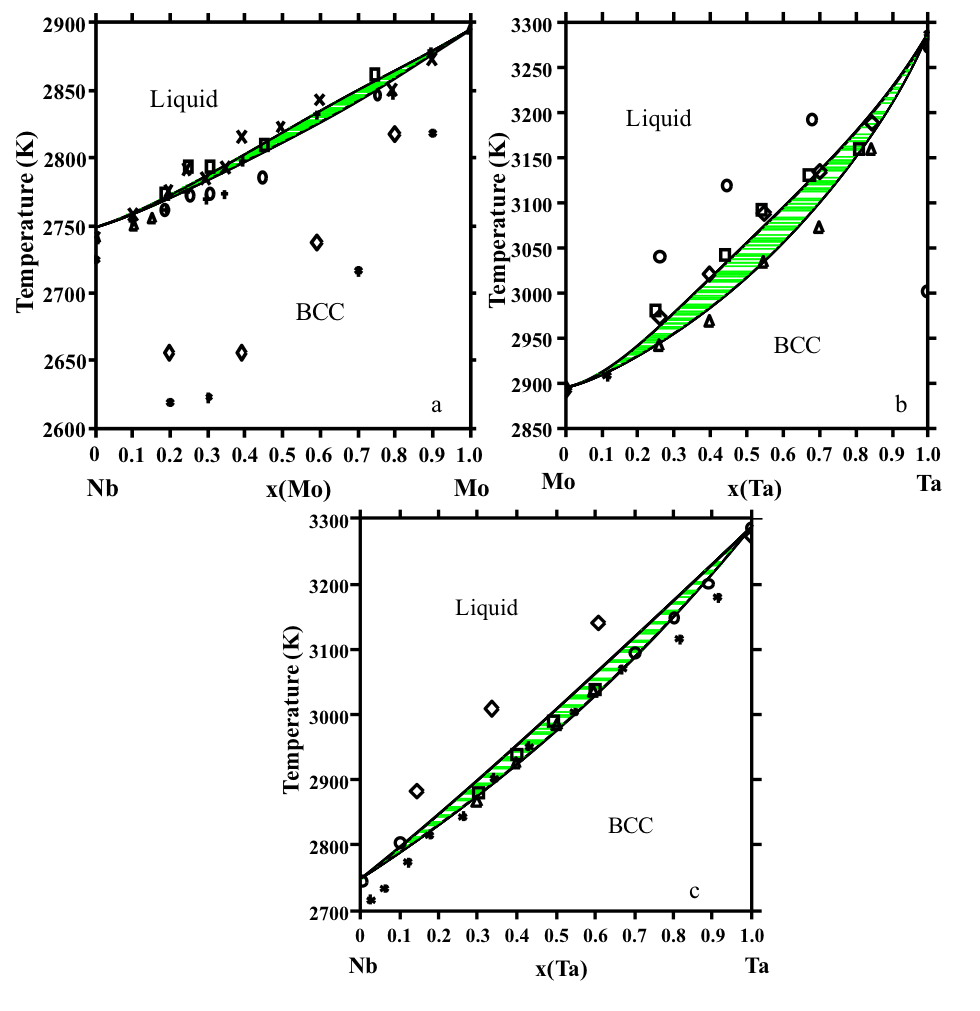
\includegraphics[width=\textwidth]{Chapter-3/Figures/binary1.png}
	\caption{Previously modeled thermodynamic descriptions of the Mo-Nb (a) \cite{Xiong2004}, Mo-Ta (b) \cite{Xiong2004} and Nb-Ta (c) \cite{Xiong2004} binary systems in comparison with available liquidus and solidus phase boundary experimental data to ensure accuracy as detailed in \cite{Xiong2004}. }
	\label{Ch3-figure:binary1}
\end{figure}
%%%

\newpage
%%%
\begin{figure}[H]
	\centering
	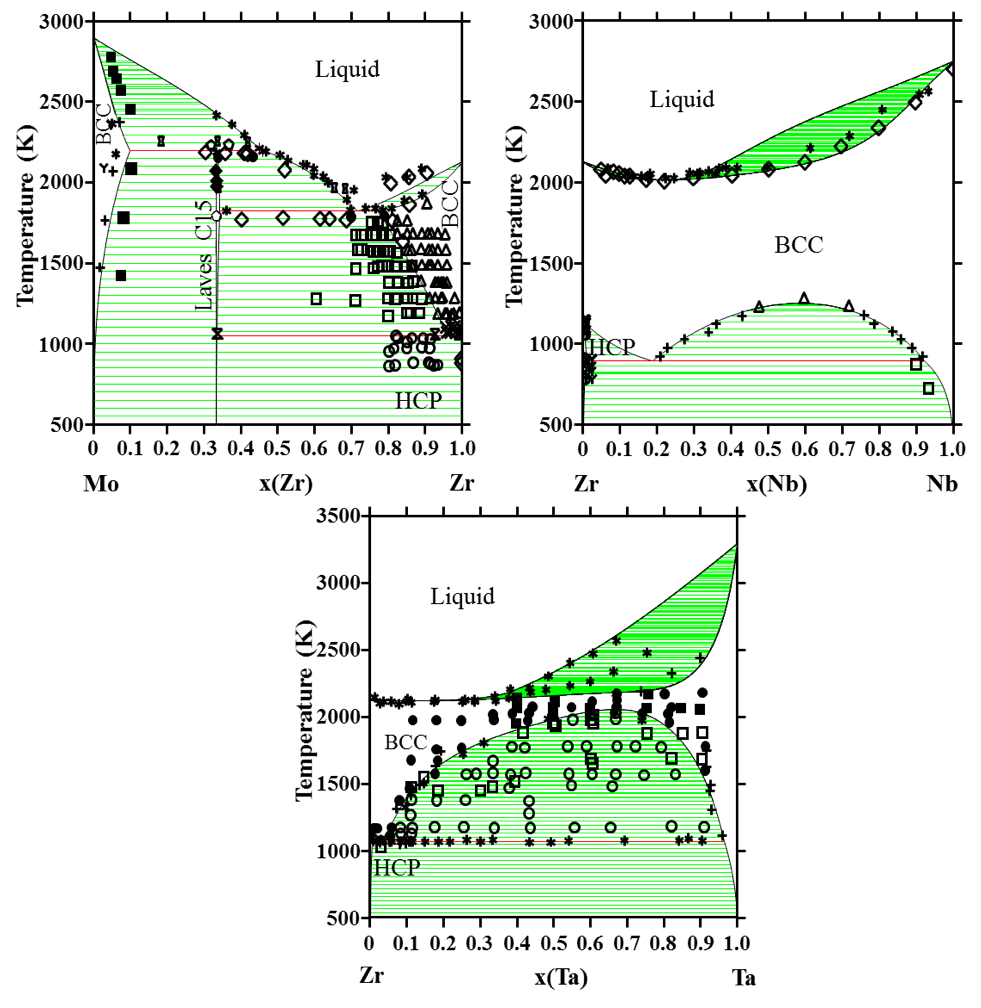
\includegraphics[width=\textwidth]{Chapter-3/Figures/binary2.png}
	\caption{Previously modeled thermodynamic descriptions of the Mo-Zr \cite{Perez2003} system is plotted with phase boundary, reaction, single phase and two phase experimental data. The previously modeled Nb-Zr \cite{Guillermet1991,Abriata1982} system is plotted with solidus, hcp solvus and bcc solvus experimental data. The previously modeled Ta-Zr \cite{Guillermet1995} system is plotted with single-phase, two-phase, phase boundary and solidus experimental data (detailed in the mentioned references).}
	\label{Ch3-figure:binary2}
\end{figure}
%%%

\newpage
%%%
\begin{figure}[H]
	\centering
	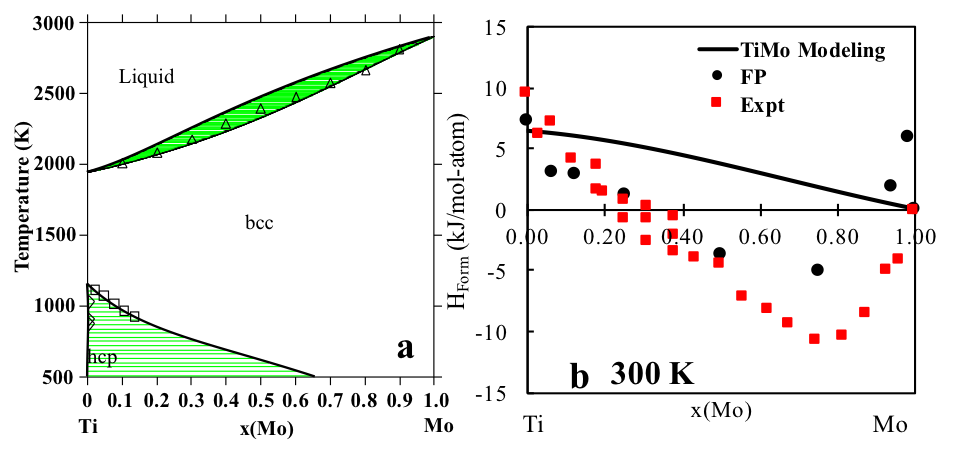
\includegraphics[width=\textwidth]{Chapter-3/Figures/TiMo.png}
	\caption{Previously modeled thermodynamic description of the Ti-Mo system versus available phase boundary and solidus experimental data to ensure accuracy \cite{Ansara1998,Murray1981} (a), and enthalpy of formation of the bcc phase predicted by the previous thermodynamic modeling (solid line) at 300 $^{\circ}$K versus the present first-principles calculations (circles) at 0 $^{\circ}$K and compared with the enthalpy of formation of the bcc phase obtained from experiments \cite{Uesugi2013} (b).}
	\label{Ch3-figure:TiMo}
\end{figure}
%%%

\newpage
%%%
\begin{figure}[H]
	\centering
	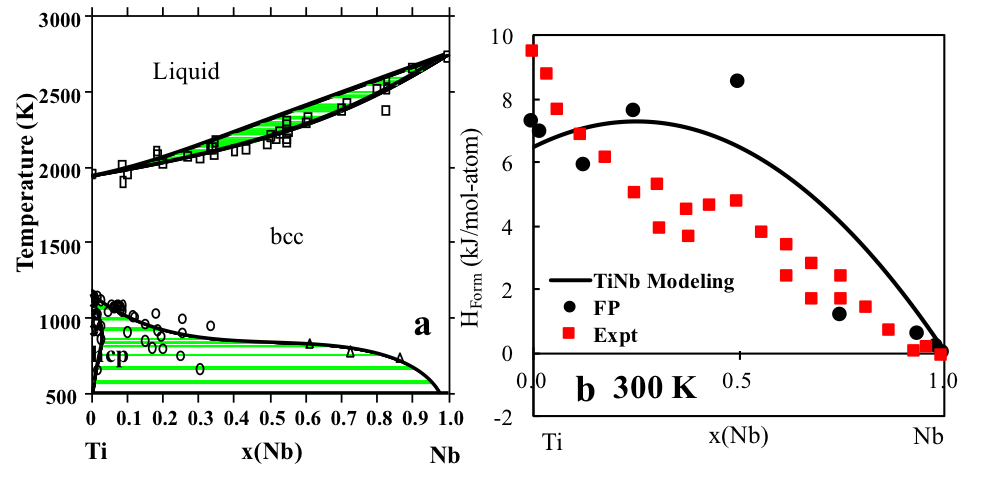
\includegraphics[width=\textwidth]{Chapter-3/Figures/TiNb.png}
	\caption{Previously modeled thermodynamic description of the Ti-Nb system versus available phase boundary and solidus experimental data to ensure accuracy \cite{Zhang2001,Kumar1994,Kumar1994a}[20,48] (a), and enthalpy of formation of the bcc phase predicted by the previous thermodynamic modeling (solid line) at 300 $^{\circ}$K versus the present first-principles calculations (circles) at 0 $^{\circ}$K compared with the enthalpy of formation of the bcc phase obtained from experiments \cite{Uesugi2013} (b).}
	\label{Ch3-figure:TiNb}
\end{figure}
%%%

\newpage
%%%
\begin{figure}[H]
	\centering
	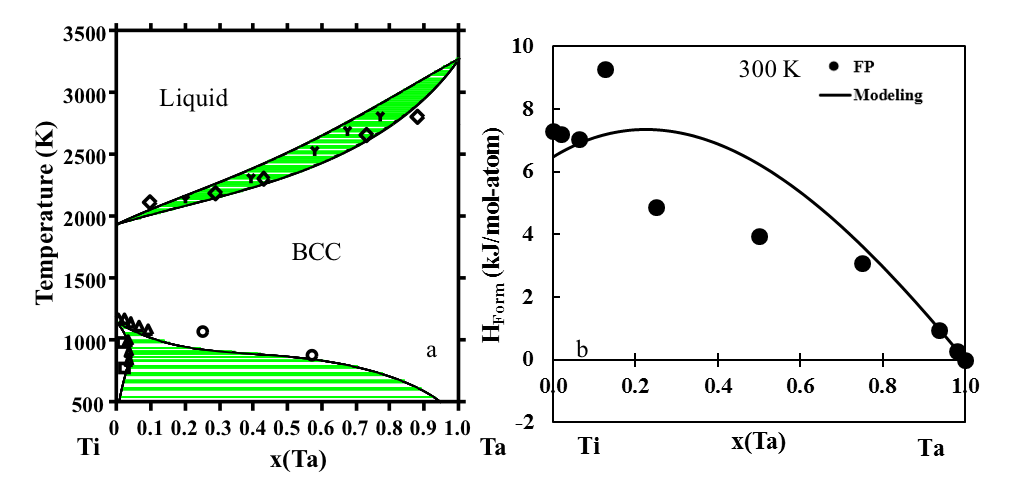
\includegraphics[width=\textwidth]{Chapter-3/Figures/TiTa.png}
	\caption{Previously modeled thermodynamic description of the Ti-Ta system versus available phase boundary and solidus experimental data to ensure accuracy \cite{Murray1987,Ansara1998} (a), and enthalpy of formation of the bcc phase predicted by the previous thermodynamic modeling (solid line) at 300 $^{\circ}$K versus the present first-principles calculations (circles) at 0 $^{\circ}$K (b).}
	\label{Ch3-figure:TiTa}
\end{figure}
%%%

\newpage
%%%
\begin{figure}[H]
	\centering
	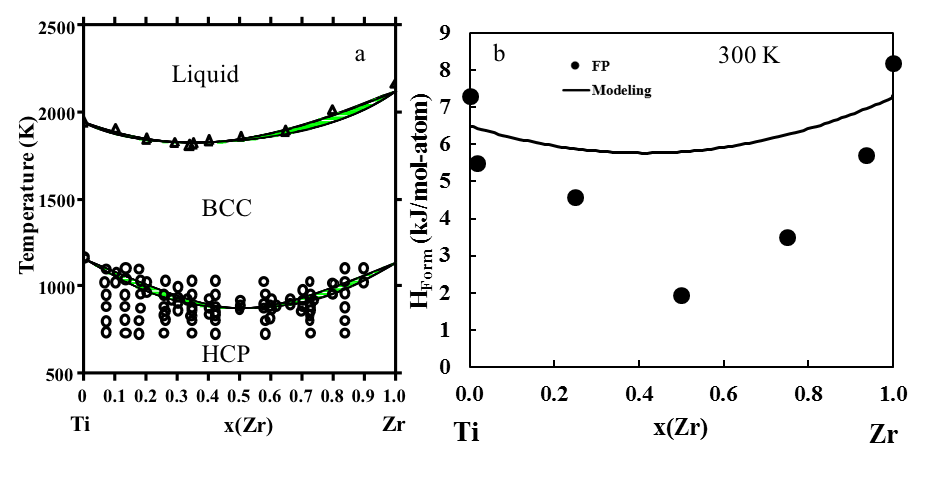
\includegraphics[width=\textwidth]{Chapter-3/Figures/TiZr.png}
	\caption{Previously modeled thermodynamic description of the Ti-Zr system versus available phase boundary and solidus experimental data to ensure accuracy \cite{Kumar1994a} (a), and enthalpy of formation of the bcc phase predicted by the previous thermodynamic modeling (solid line) at 300 $^{\circ}$K versus the present first-principles calculations (circles) at 0 $^{\circ}$K (b).}
	\label{Ch3-figure:TiZr}
\end{figure}
%%%

\newpage
%%%
\begin{figure}[H]
	\centering
	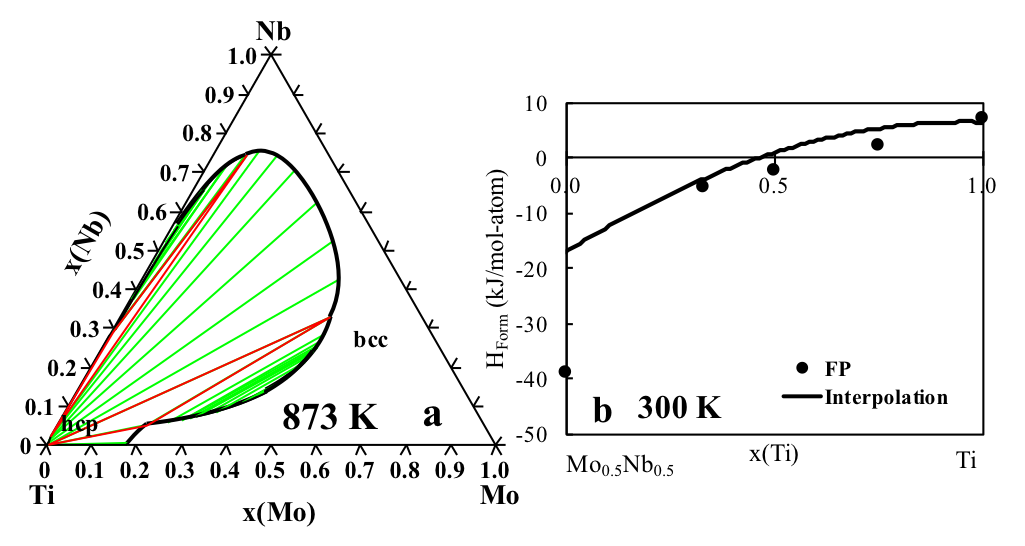
\includegraphics[width=\textwidth]{Chapter-3/Figures/TiMoNb.png}
	\caption{Binary interpolation of the isothermal section of the Ti-Mo-Nb system plotted at 873 $^{\circ}$K (a), and enthalpy of formation of the bcc phase predicted by the binary interpolation of the thermodynamic modeling (solid line) at 300 $^{\circ}$K versus the present first-principles calculations (circles) at 0 $^{\circ}$K (b).}
	\label{Ch3-figure:TiMoNb}
\end{figure}
%%%

\newpage
%%%
\begin{figure}[H]
	\centering
	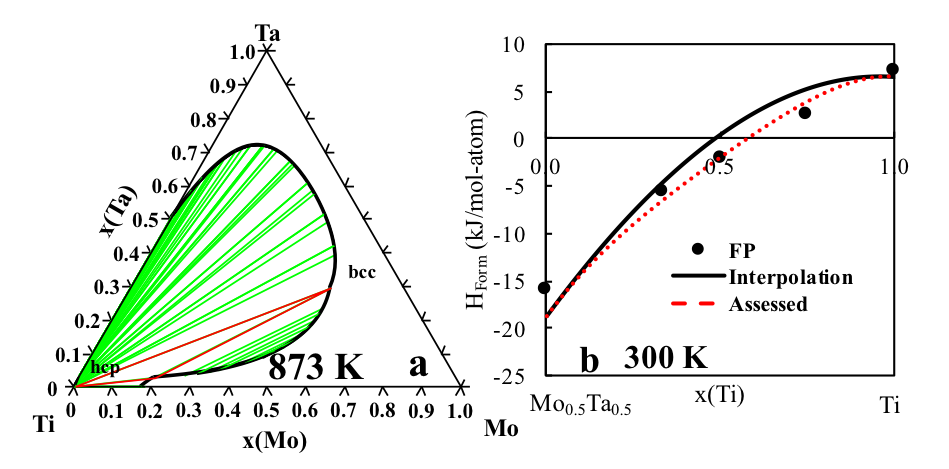
\includegraphics[width=\textwidth]{Chapter-3/Figures/TiMoTa1.png}
	\caption{Binary interpolation of the isothermal section of the Ti-Mo-Ta system plotted at 873 $^{\circ}$K (a), and enthalpy of formation of the bcc phase predicted by the previous thermodynamic modeling (solid line) at 300 $^{\circ}$K and the ternary assessed thermodynamic modeling (red dotted line) versus the present first-principles calculations (circles) at 0 $^{\circ}$K (b).}
	\label{Ch3-figure:TiMoTa1}
\end{figure}
%%%

\newpage
%%%
\begin{figure}[H]
	\centering
	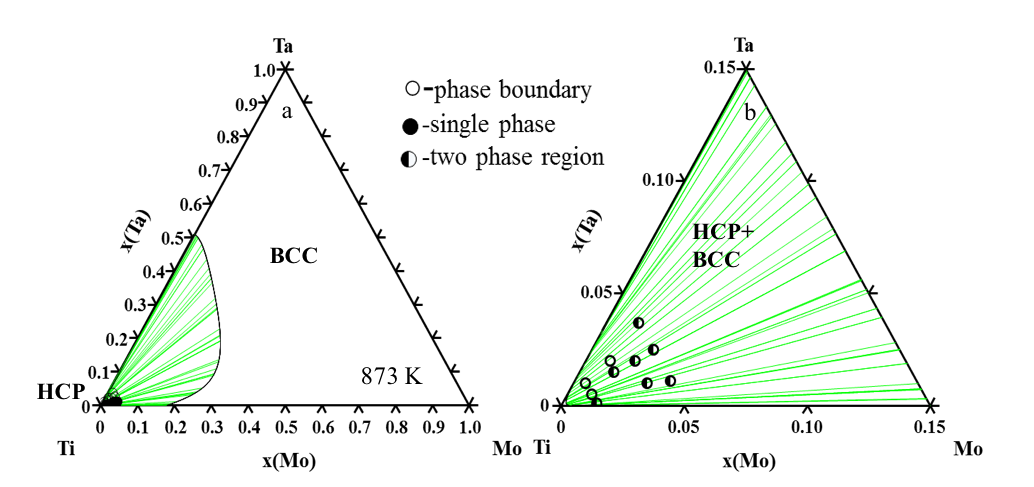
\includegraphics[width=\textwidth]{Chapter-3/Figures/TiMoTa2.png}
	\caption{Ternary assessed isothermal section of the Ti-Mo-Ta system plotted at 873 $^{\circ}$K (a), and zoomed in ternary assessed isothermal section at 873 $^{\circ}$K with the phase boundary and two-phase region experimental data \cite{Nikitin1971} (b) to ensure accuracy of the ternary assessment.}
	\label{Ch3-figure:TiMoTa2}
\end{figure}
%%%

\newpage
%%%
\begin{figure}[H]
	\centering
	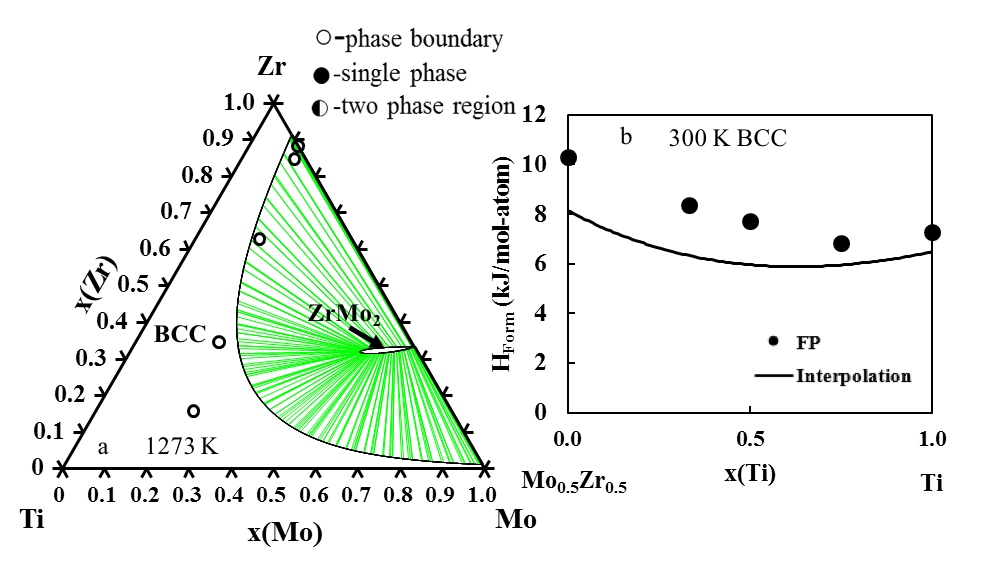
\includegraphics[width=\textwidth]{Chapter-3/Figures/TiMoZr.png}
	\caption{Binary interpolation of the isothermal section of the Ti-Mo-Zr system plotted at 1273 $^{\circ}$K compared with experimental phase boundary data \cite{Kar2008,Prokoshkin1967} (a), and enthalpy of formation of the bcc phase predicted by the previous thermodynamic modeling (solid line) at 300 $^{\circ}$K versus the present first-principles calculations (circles) at 0 $^{\circ}$K (b).}
	\label{Ch3-figure:TiMoZr}
\end{figure}
%%%

\newpage
%%%
\begin{figure}[H]
	\centering
	\includegraphics[width=\textwidth]{Chapter-3/Figures/TiNbTa1.png}
	\caption{Binary interpolation of the isothermal section of the Ti-Nb-Ta system plotted at 673 $^{\circ}$K compared with experimental phase boundary data \cite{Na2001} (a), and binary interpolation of the isothermal section of the Ti-Nb-Ta system plotted at 823 $^{\circ}$K compared with experimental phase boundary data \cite{Na2001} (b).}
	\label{Ch3-figure:TiNbTa1}
\end{figure}
%%%

\newpage
%%%
\begin{figure}[H]
	\centering
	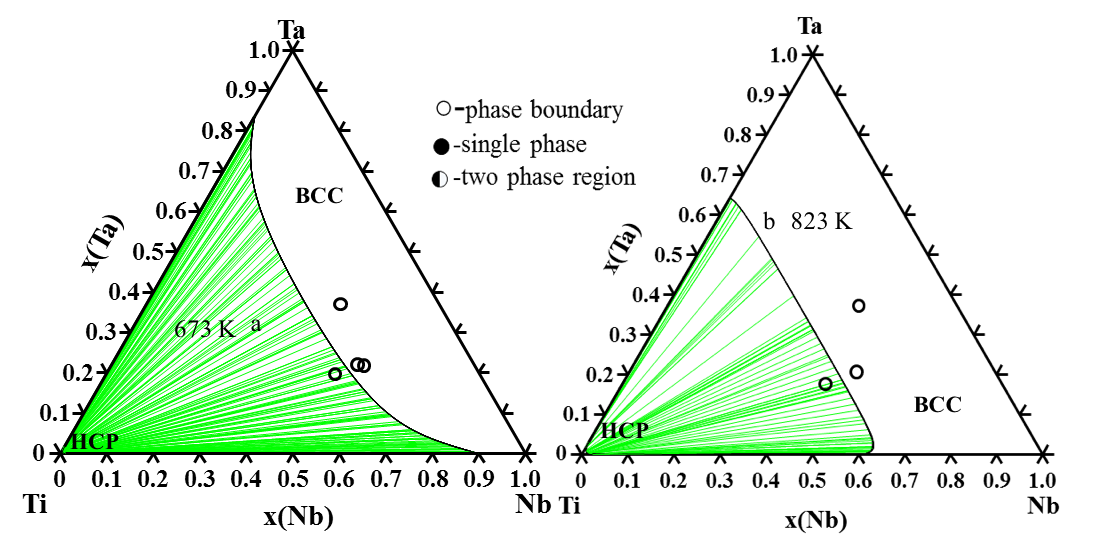
\includegraphics{Chapter-3/Figures/TiNbTa2.png}
	\caption{Enthalpy of formation of the bcc phase predicted by the previous thermodynamic modeling (solid line) at 300 $^{\circ}$K and the ternary assessed thermodynamic modeling (red dotted line) versus the present first-principles calculations (circles) at 0 $^{\circ}$K.}
	\label{Ch3-figure:TiNbTa2}
\end{figure}
%%%

\newpage
%%%
\begin{figure}[H]
	\centering
	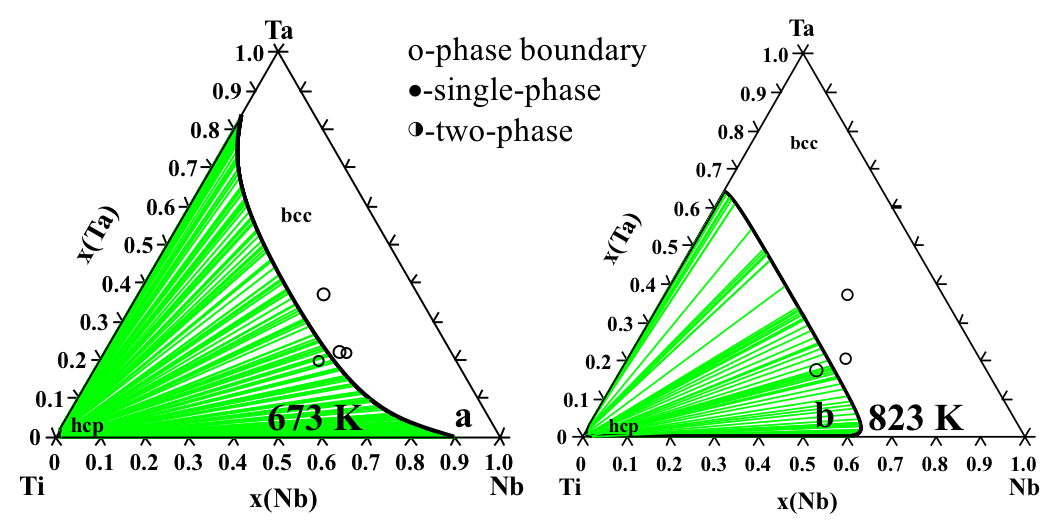
\includegraphics[width=\textwidth]{Chapter-3/Figures/TiNbTa3.png}
	\caption{Ternary assessed isothermal section of the Ti-Nb-Ta system plotted at 673 $^{\circ}$K compared with experimental phase boundary data \cite{Na2001} to ensure accuracy of the ternary assessment (a), and ternary assessed isothermal section at 823 $^{\circ}$K compared with experimental phase boundary data \cite{Na2001} to ensure accuracy of the ternary assessment (b).}
	\label{Ch3-figure:TiNbTa3}
\end{figure}
%%%

\newpage
%%%
\begin{figure}[H]
	\centering
	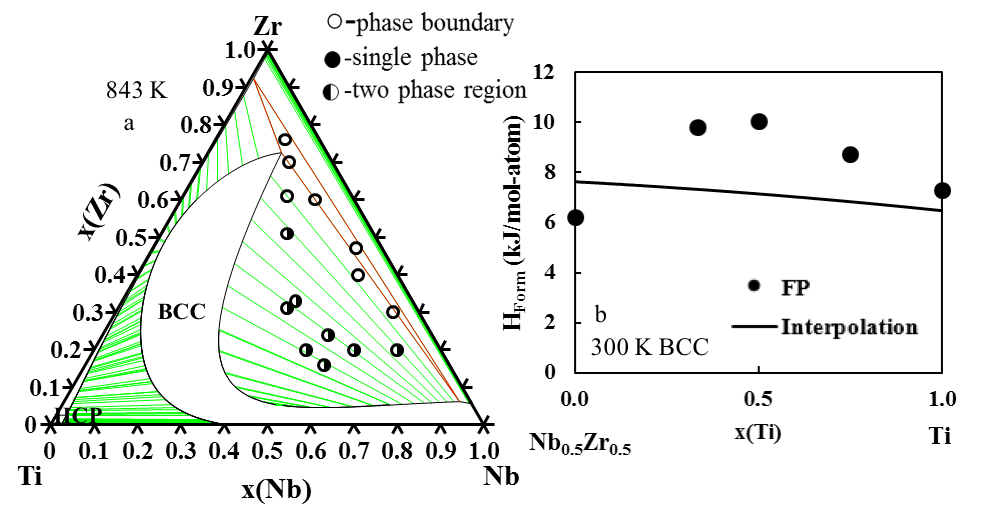
\includegraphics[width=\textwidth]{Chapter-3/Figures/TiNbZr.png}
	\caption{Binary interpolation of the isothermal section of the Ti-Nb-Zr system plotted at 843 $^{\circ}$K compared with experimental phase boundary and two-phase region data \cite{Tokunaga2007} (a), and enthalpy of formation of the bcc phase predicted by the previous thermodynamic modeling (solid line) at 300 $^{\circ}$K versus the present first-principles calculations (circles) at 0 $^{\circ}$K (b).}
	\label{Ch3-figure:TiNbZr}
\end{figure}
%%%

\newpage
%%%
\begin{figure}[H]
	\centering
	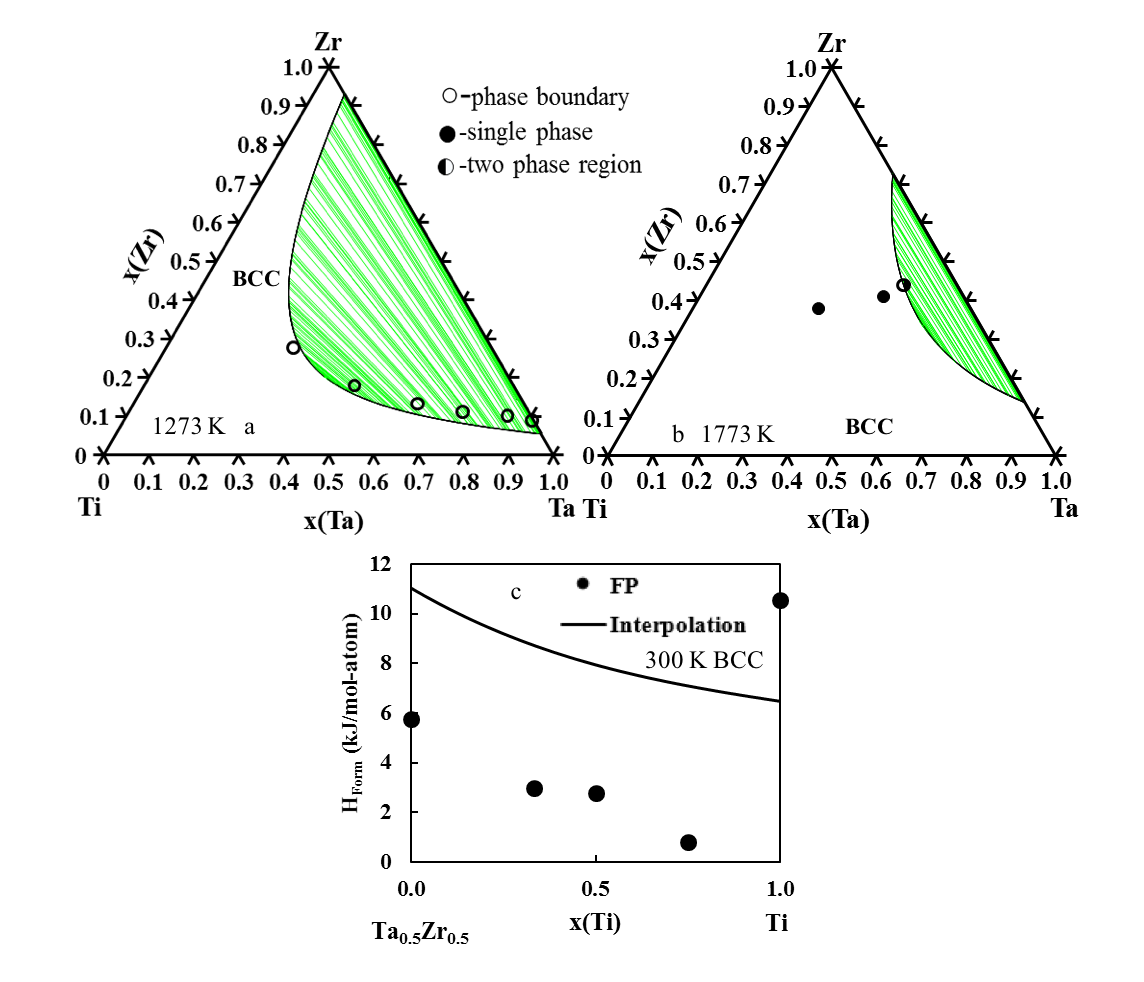
\includegraphics[width=\textwidth]{Chapter-3/Figures/TiTaZr1.png}
	\caption{Binary interpolation of the isothermal section of the Ti-Ta-Zr system plotted at 1273 $^{\circ}$K compared with experimental phase boundary data \cite{Lin1996,Hoch1964} (a), and binary interpolation of the isothermal section of the Ti-Ta-Zr system plotted at 1773 $^{\circ}$K compared with compared with experimental single phase and two-phase region data \cite{Lin1996,Hoch1964} (b).}
	\label{Ch3-figure:TiTaZr1}
\end{figure}
%%%

\newpage
%%%
\begin{figure}[H]
	\centering
	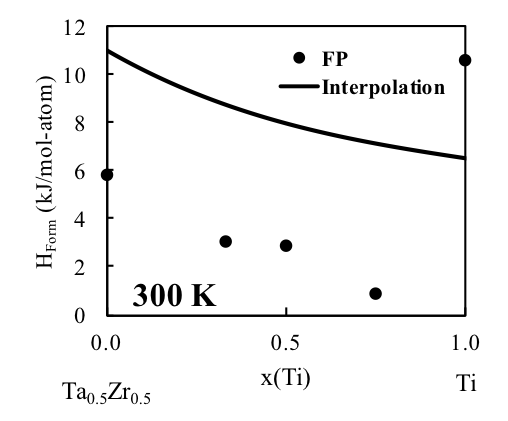
\includegraphics{Chapter-3/Figures/TiTaZr2.png}
	\caption{Enthalpy of formation of the bcc phase predicted by the previous thermodynamic modeling (solid line) at 300 $^{\circ}$K versus the present first-principles calculations (circles) at 0 $^{\circ}$K.}
	\label{Ch3-figure:TiTaZr2}
\end{figure}
%%%